%Original version in April 2002 by Antje Endemann
%
%Adapted for usage in Student Conference course by jubo (050118).
%Optimized for usage with pdflatex. For usage with plain latex,
%figures must be in Postscript (.ps or .eps files) and additional
%packages must be imported.
%Last updated 100105 by jubo
%
%This template works for outline and annotated bibliography
%(deliverable 2) without any changes.
%For usage with full and final papers (deliverables 3 and 4a/b)
%you must make several changes. All necessary changes are
%described in three specific commented sections preceded by
%`%%%%% BEGIN OF ADJUSTMENTS SECTION %%%%%'.
%The changes are in order of appearance:
%   - adjust the `\documentclass' command
%   - uncomment the abstract section
%   - adjust the `\bibliographystyle' command

%%%%% BEGIN OF 1st ADJUSTMENTS SECTION %%%%%
% You must use only one of the following `\documentclass' commands
% For the outline and annotated bibliography (deliverable 2)
% you must use the following command:
%
% \documentclass[runningheads,a4paper,oribibl]{llncs}
%
% For the full and final paper (deliverables 3 and 4a/b)
% you must use the command below (and put the one above in comments).
% In other words, the 'oribib' option must be used for Deliverable 2
% but not for 3 and 4a/b.
% 
%
\documentclass[runningheads,a4paper]{llncs}
%
%%%%% END OF 1st ADJUSTMENTS SECTION %%%%%

\usepackage[T1]{fontenc}  %% needed for special characters (umlaut)
\usepackage[utf8]{inputenc}
\usepackage{graphicx}     %% for graphical things such as including pictures
\usepackage{url}          %% for proper formatting of URLs

% Albins Packages
\usepackage{array}

%
\begin{document}

\pagestyle{headings}

\mainmatter

% \title{Guidelines for Designing Touch Interfaces for Controlling Robotic Nozzles in Critical Emergency Situations.}

\title{Can a High Color Contrast Touch Interface Increase User Reaction Time when Using a Smart Phone Web Based Application?}

% response
% reaction time

% The abbreviated title will be shown in the headers of even pages.
% You should use the full title unless it is too long.

% \titlerunning{Touch Interfaces for Robotic Nozzles in Emergency Situations}

\titlerunning{Can High Color Contrast Increase User Reaction Time}

\author{Albin Hübsch}

\institute{
	Department of Computing Science \\
	Umeå University, Sweden \\
	\email{albin.hubsch@gmail.com} \\
	\url{http://albinhubsch.se}
}

\maketitle

%%%%% BEGIN OF 2nd ADJUSTMENTS SECTION %%%%%
% Do NOT include an abstract in the outline and annotated bibliography
% (deliverable 2). For the full and final paper (deliverables 3 and 4a/b),
% you must uncomment the following two commands and place your text for
% the abstract in between them.
%
\begin{abstract}
This study aims to investigate if it is possible to receive better user performance when using a high-color-contrast compared to a low-color-contrast touch screen interface in a mobile web application. The performance was measured by combining the time each user took to respond to instructions (reaction time) and the number of input errors the user made. Received test data appeared to be corrupt, most probably due to limitations in web application technology, despite this our result show that the low color contrast interface produced 475\% more user input errors compared to the high color contrast interface. No difference in reaction time could be found between the two versions.
\end{abstract}
%
%
%This study aims to investigate if there is a performance difference between a high color contrast and a low color contrast touch screen interface. The performance was measured by combining the time each test subject took to respond on instructions (reaction time) and the number of input errors. The result shows that the high color contrast interface resulted in significantly fewer user input errors. There was no differences in reaction time between the two interfaces.
%%%%% END OF 2nd ADJUSTMENTS SECTION %%%%%

\section{Introduction}
The main goal with this paper is to evaluate if color contrast has a significant impact on usability in web based smart-phone applications. Consumer touch screen devices such as smart-phones have rapidly increased in number and availability recent years. The touch screen technology has made great advances~\cite{jennings2013touch} and it is frequently used as a way of receiving user input. When this technology moves to a broader audience, higher demands on usability needs to be set~\cite{gong2004guidelines}. To further explore how usability can be improved using touch screen technology we have in this paper investigated if reaction time (the time it takes for a user to react on instructions, further referred to as RT in this paper) and user input errors (the number of user input errors when interacting with a system, further referred to as UIE in this paper) can reach better results by increasing color contrast within the interface. With "better results" we mean fewer UIEs and faster RTs. Increased number of user input errors means that users repeatedly presses the wrong buttons which tells us that it is hard to accomplish desired tasks. Faster reaction times does not necessarily mean "better", but in this experiment we had tasks that should be performed as fast as possible which led us to the conclusion, faster reaction times are "better".

Contrast is determined by the difference in color and brightness of an object and objects within the same field of view. High contrast is the degree of difference between dark and light when it approaches the maximum possible difference. Low contrast is the opposite, low difference between dark light.

Earlier studies completed in this field have explored how we perceive different color contrast and how it can affect our reading performance~\cite{wu2003improving}. It has also been proved that chromaticity, contrast, and cone opponency in color space can affect RTs~\cite{mckeefry2003simple}. Many best practices for mobile development have also shown that "requirements for sufficient color contrast"~\cite{marcus2013design} must be met to best amplify the content. Still the question remains, can a high color contrast interface increase the the reaction time and decrease the amount of user input errors?

High RTs and low UIEs are especially desirable when designing user interfaces for situations with high demands on quick user input and low error tolerance such as in emergency situations. The results of studies like this are especially useful for designers and front end developers.

\section{Method}
In order to be able to test if color contrast has a substantial impact on the RT and UIE of a touch screen user interface we have designed a simple web application for an Android smart-phone. The application exists in two versions, one with low color contrast (referred to as LCC in this paper) and one with high color contrast (referred to as HCC in this paper) interface as can be seen in Fig~\ref{fig:application}. We conducted an A/B test to measure the performance difference between the versions.

\begin{figure}
	\centering
	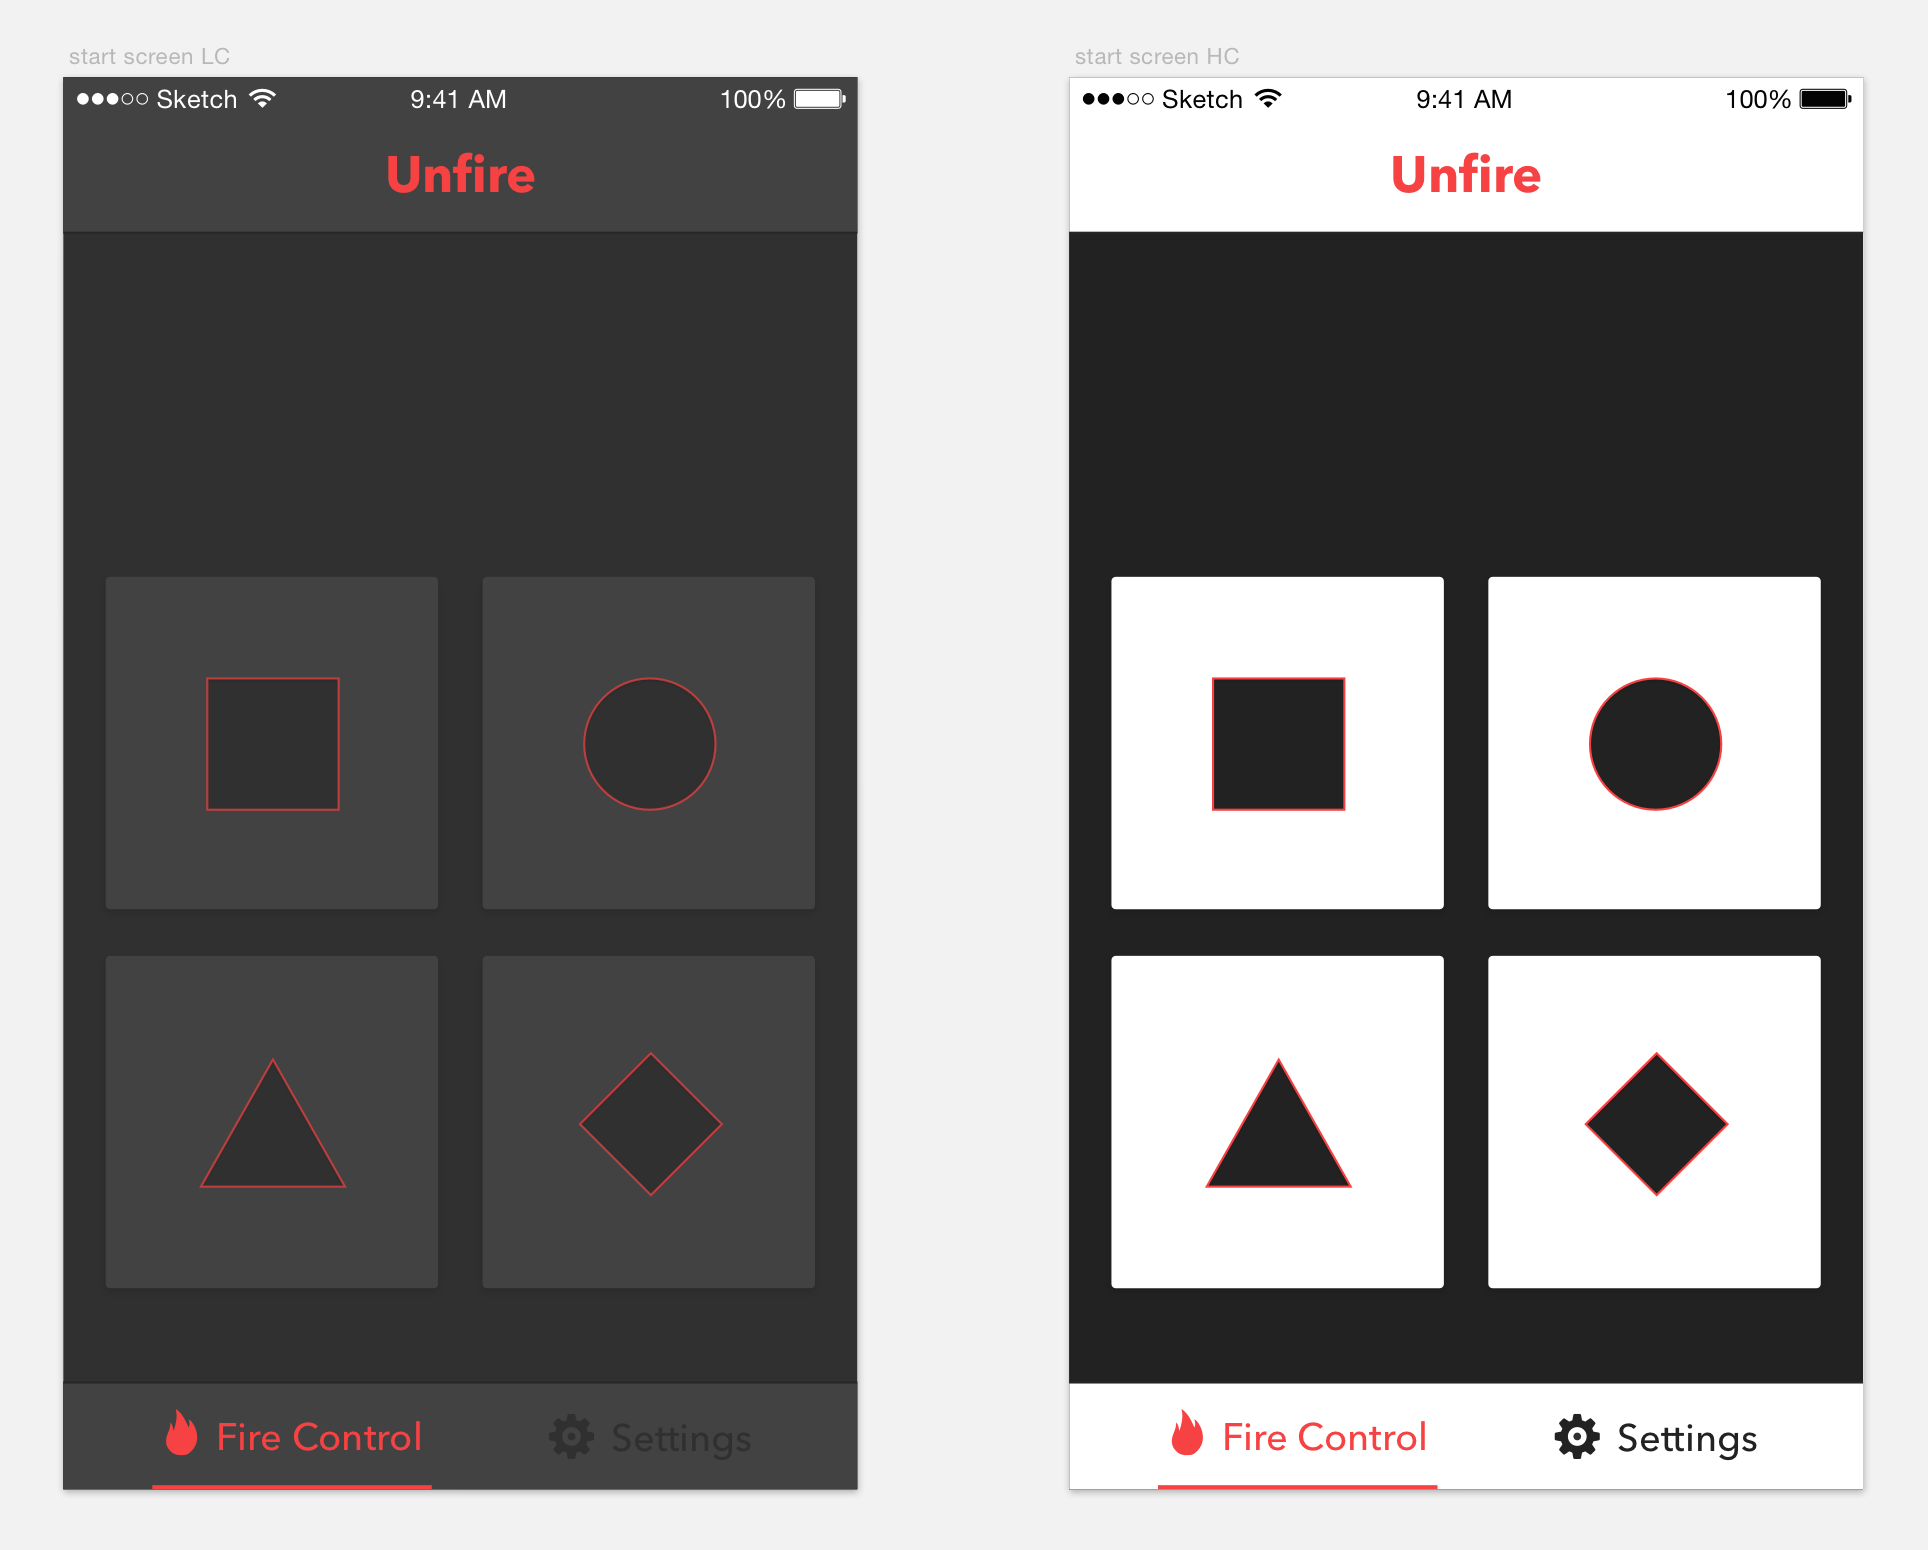
\includegraphics[width=\textwidth]{application}
	\caption{Our two versions of the application designed with different contrast. To the left the low contrast interface and to the right the high contrast interface. The application and its interface was designed specifically for this test. The bottom menu was added to give the interface more of a complete application feel. 
	\label{fig:application}}
\end{figure}

We designed the application by following design guidelines introduced and presented here~\cite{hoober2011designing,johnson2013designing,gong2004guidelines,norman2013design}. These guidelines can be seen as a set of rules to follow when designing any kind of user interface. We used guidelines to get proper sized buttons, good spacing between content and best positioning of navigation.

\subsection{Designing the A/B test}
We conducted an A/B test to measure the differences in RT and UIE between the two versions. An A/B test is a commonly used method by developers and designers to test differences in performance between applications when the differentiated factors are known~\cite{johnson2013designing}. Where in this case our known factor is the contrast difference. 

The application consists of 4 buttons\footnote{On-screen button}, each button representing a function. To differentiate each button from the others we put a unique shape in each button. The shapes we used were a, square, circle, triangle and a rhomb (Fig~\ref{fig:application}).

To be able to give the test persons consistent instructions through the complete test we designed a program that presented the instructions on a secondary screen. 
\begin{figure}
	\centering
	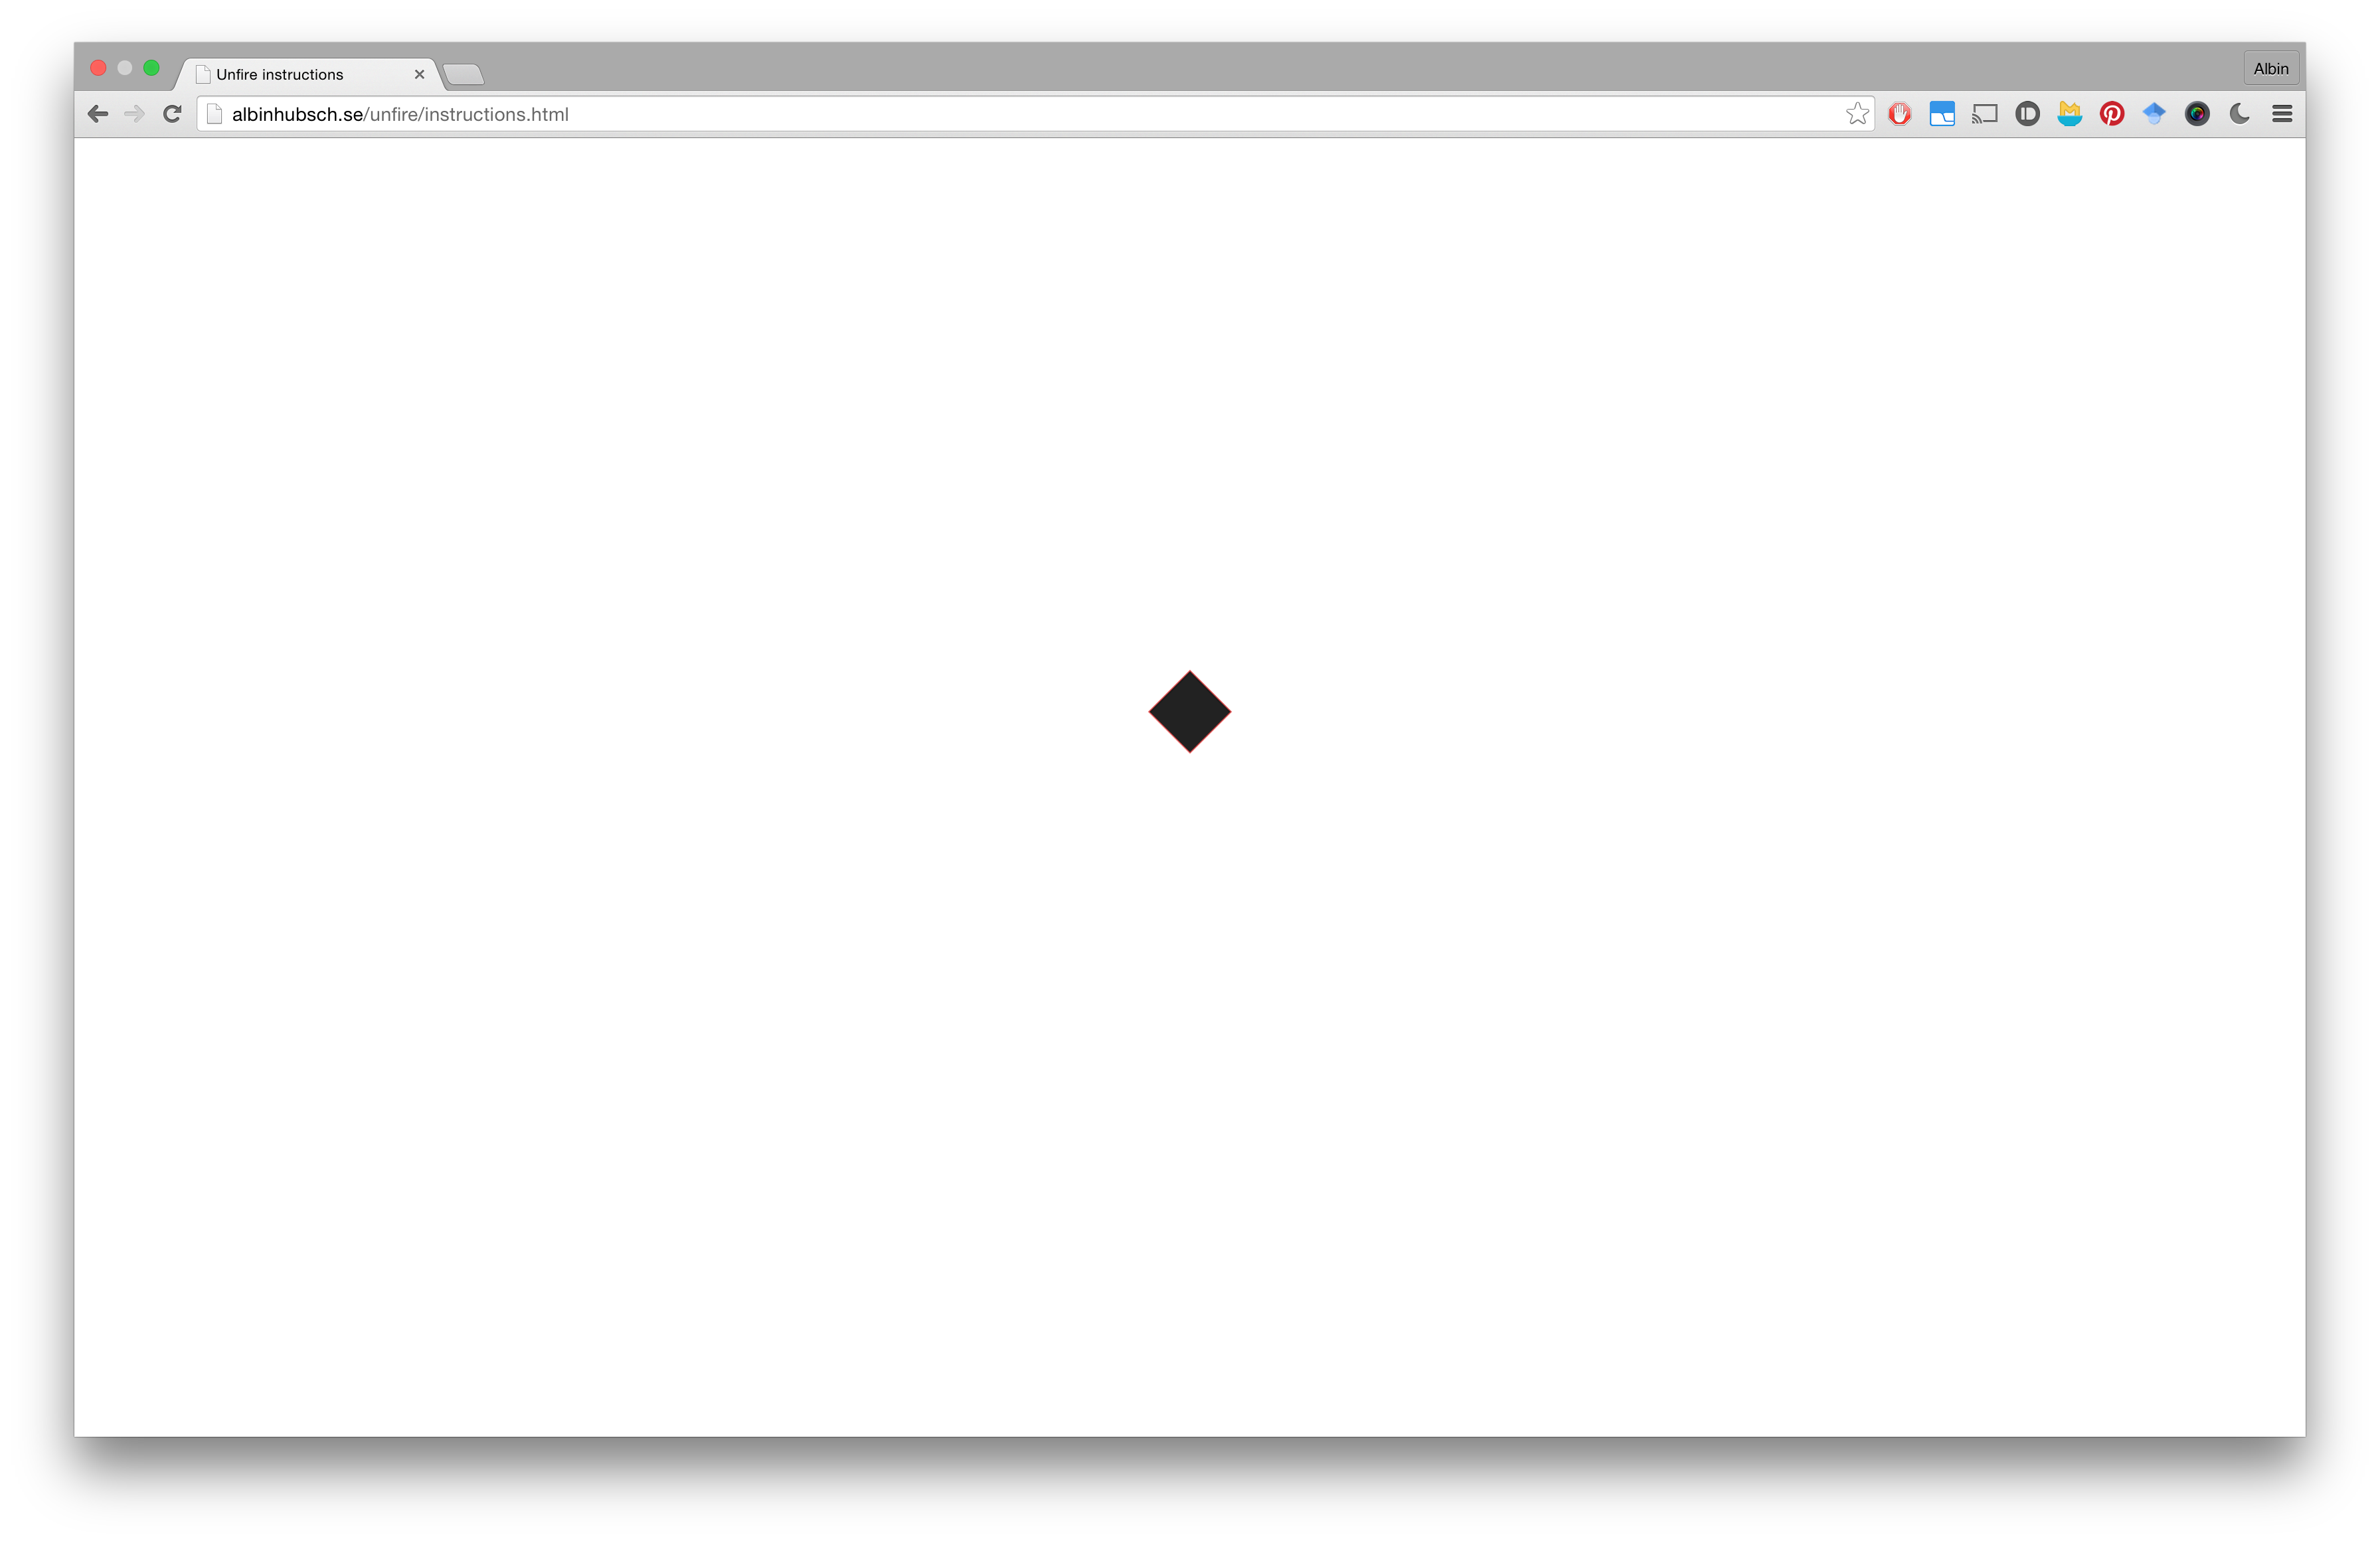
\includegraphics[width=\textwidth]{instructions}
	\caption{Our program designed to present user instructions. Instructions were given in a series of 20. Between each instruction there was a delay set to be between 2.5 and 4 seconds. Each time a new symbol where showed a timestamp were logged in a unique user instruction file.
	\label{fig:instructions}}
\end{figure}
The instructions were a series of 20 instructions with shapes identical to the ones in the application buttons. The test persons were told to press the representative shape in the application as fast as they could in order to measure the reaction time. If they realized that they pressed the wrong button they were just told to continue the test by pressing the right button as fast as they realized. the application registered all wrong, non-matching input as an UIE. Each test was performed indoors with varying surroundings such as different lightning conditions and noise levels. 

We tested each version of the application on five persons, all within the same age group (20-30) and with a variety of backgrounds. In total we got 10 test results with a gender split of 50\% women and 50\% men that grouped into LCC and HCC. We analyzed them against each other to measure if any differences in RT or UIE between the two versions could be statistically confirmed.

\subsection{Evaluation of the A/B test}
Our data received from the tests consisted of UNIX timestamps\footnote{More info at: \url{http://www.unixtimestamp.com/}} measured in milliseconds. Each time the user interacted with the application it registered which button that was pressed and saved it together with a timestamp. Equally, every time the instruction program showed a new symbol it logged the symbol together with a timestamp. As a result we received two data sets of symbols with corresponding timestamps for each test person, resulting in a total of 200 records. Although the data was hard to interpret due to its compact look, a python script was written to structure the resulting timestamps into a more readable format. We calculated each RT by subtracting the timestamp when the instruction was given from the registered user input timestamp. Out of this we could calculate the mean RT for both groups LCC and HCC. The calculation of RT did not take in consideration if user input was a match with the instruction or not. It was still considered as a reaction.

UIEs were counted every time the user pressed a non matching object compared to the one given in the instructions. All input errors in each group, LCC and HCC, were counted to see if one of the groups produced more UIEs.

\section{Result}
From our results we can not draw any statistically significant conclusions about differences in reaction time between the two groups high color contrast and low color contrast. This is most probably due to corrupt test data, a result from limitations in web application technology, see Section \ref{sec:discussion}. With user input errors we found that the low color contrast group produced significantly more user input errors than the hight color contrast group.

\subsection{Reaction Times (RT)}
Table~\ref{tab:groupRT} shows the average reaction time and standard deviation for each group. According to the results people in the high color contrast group had insignificant slower reaction times compared to the ones in the low color contrast group.

\begin{table}[]
	\centering
	\setlength{\tabcolsep}{1em}
	\setlength\extrarowheight{1em}
	\begin{tabular}{l|l|l}
		\textbf{} & \textbf{Average RT} & \textbf{Standard Deviation} \\ \hline
		\textbf{HCC} & 783 ms & 969 ms \\ \hline
		\textbf{LCC} & 550 ms & 1393 ms
	\end{tabular}
	\caption{Average reaction time and standard deviation for each group, low color contrast and high color contrast. A two tailed t-test was performed on the two groups and showed that no significant difference could be determined between them.
	\label{tab:groupRT}}
\end{table}

To check if the RTs in the two groups are significantly different we assumed the two data sets where normal distributed based on the n>30 preference, and performed a two tailed t-test. The test produced a p-value of 0.17 which is bigger than a desired error margin ($\alpha$) of 5\%. This shows that the difference in RT between the two groups is not statistically significant. Regardless what the t-test says our standard deviations are indicating that something might be wrong with our data (see section \ref{sec:discussion}).

\subsection{Input Errors (IE)}\label{subsec:InputErrors}
None of the groups where completely free from user input errors. As can be seen in Table~\ref{tab:userIE}, users that were given the LCC interface produced 475\% more UIE than the HCC group.

\begin{table}[]
	\centering
	\setlength{\tabcolsep}{1em}
	\setlength\extrarowheight{1em}
	\begin{tabular}{l|l|l|l}
		\textbf{} & \textbf{Errors} & \textbf{Standard Deviation} & \textbf{Errors/User} \\ \hline
		\textbf{HCC} & 4 & 1.10 & 0.8 \\ \hline
		\textbf{LCC} & 19 & 3.49 & 3.8
	\end{tabular}
	\caption{Number of user input errors registered in each group and a calculation of input errors per user in each group. The low color contrast interface produced 475\% more input errors compared to the high color contrast version. A two tailed t-test also showed that there is a significant difference between the two versions. A high color contrast interface can therefore be a preferred design method if a low amount of user input error is desired.
	\label{tab:userIE}}
\end{table}

Table~\ref{tab:userIE} shows us that the users in the HCC group generally had a more stable and consistent performance compared to the LCC group. We also performed a two tailed t-test on the UIE data set. The outcome of this test was a p-value of 0.001 which is significantly smaller than a $\alpha$ of 5\% telling us that the HCC group performed better.

\section{Discussion}\label{sec:discussion}
From our test results we cannot draw any conclusions about differences in reaction time between the high color contrast interface and the low color contrast interface. However we could see that the high color contrast interface was more reliable in performance when it comes to the amount of user input errors, according to our results. 

What we have seen in our collected test data can strongly negotiate the legibility of the results. The calculated standard deviations gave us hints on that something was wrong. We dug deeper into each test persons results and found that the data must be corrupt. We found that we had randomly received negative RTs which in theory should be completely impossible. We were prepared that the timestamps could be off sync due to individual system clocks and no boot up pairing. However this would only have resulted in a consistent off sync. Instead we got inconsistent hiccups in our timestamps. We suspect this is a result from either hardware limitations or limitations in the JavaScript\footnote{A prototype based dynamic scripting language} engine for web applications on Android.

Although we can not draw any conclusions out from the results we have learned that smart phone web based applications should only be used if sometimes slow technology, user input errors and long reaction times from the user can be accepted. The HCC interface could also be seen as a preferred design method, even if the data was corrupt, because the users performed more consistent with UIEs compared to the users in the LCC group, see number of UIEs and their standard deviations in~\ref{subsec:InputErrors}.

\subsection{Drawbacks and Limitations}\label{subsec:drawbacks}
The main drawback of this study is the corrupt data set. This has to be in mind when we draw any conclusions out of the results. The problem could most probably be solved by simply rerunning the complete test using a native smart phone application instead of a web based solution.

Each test person performed only one test with a supervisory selected interface, the LCC or HCC version. To eliminate possible affecting surrounding factors each person should have done the test several times and with both the LCC and HCC interfaces. This would also have made it possible to recognize if the test persons memorized the patterns in any way.

\begin{description}
	\item[Small test group.] To be able to get a more statistical valid result the test group has to be bigger. A good rule of thumb is at least 30.
	\item[Many affecting parameters.] The prototype is simple in its appearance but there are still many parameters that can affect the users interaction and their RTs. Icons, icon size, optimal number of on screen buttons, size of hand-held device etc. All this, and more, should have been researched and taken into account if done again. 
	\item[Limited test environment.] Our tests were made using an Android based smart-phone\footnote{OnePlus Two \url{https://oneplus.net/2}} and the application was made using HTML5\footnote{HyperText Markup Language, markup standard for WWW}, CSS3\footnote{Cascading Style Sheet, styling standard for WWW} and JavaScript. We can not surely imply, without testing, that we would get the same results on an iPhone or any other smart-phone, or even with a native application.
\end{description}

\subsection{Future Work}
Due to the failed data set that we received in this paper there are things that could be improved or continued to be worked on. 
We do have some concrete suggestions that could be case for future work. 

\begin{itemize}
	\item Perform tests using a native application.
	\item Extend the test group with more test subjects. It is possible to think that the patterns that slightly appeared in our results will appear even more significant with a larger group of test subjects.
	\item Our collected test data can be downloaded\footnote{Download here~\url{https://goo.gl/x8URSB}} and used freely to investigate other aspects not mentioned in this paper. One proposal is to look at the different shapes and try to detect possible error patterns between them. Is the rhomb more frequently a case for IE compared to the other shapes?
	\item Do our results apply on other systems and techniques? Our tests are limited to the Android system and a web based application solution. It remains to answer if our results applies on all other systems. This is also a way of isolating some of the affecting parameters mentioned in Section~\ref{subsec:drawbacks}.
\end{itemize}

\section{Acknowledgments}
The author would like to thank the peer reviewers who provided valuable comments on both the content and structure of this paper.

%%%%% BEGIN OF 3rd ADJUSTMENTS SECTION %%%%%
% For the outline and annotated bibliography (deliverable 2)
% you must use the following two commands:
%
% \nocite{*}  % Includes ALL entries from the .bib-file, even if they are
            % not '\cite{}'-ed in the text above
% \bibliographystyle{plain-annote}
%
% For the full and final paper (deliverables 3 and 4a/b)
% use ONLY the following commands (i.e. put the commands above into
% comments and uncomment the command below):
%
\bibliographystyle{splncs}
%
%%%%% END OF ADJUSTMENTS SECTION %%%%%

\bibliography{Bibliography}

\end{document}
